\documentclass[border=5pt,tikz]{standalone}
\usepackage[T1]{fontenc}
\usetikzlibrary{shapes}

%\renewcommand{\familydefault}{pr4uh-1em}


\begin{document}

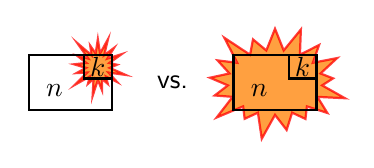
\begin{tikzpicture}
\node[starburst, thick, draw, minimum width=1cm, minimum height=.3cm,red,fill=orange,scale=.5,opacity=.75] at (.35,.2) {$\phantom{k}$};  

	\node[rectangle,minimum width=3em, minimum height=2em, inner sep=0mm, draw=black,thick] at (0,0) (nk) {};

	\node[rectangle, draw=black, thick, inner sep=0mm, minimum height=3mm, minimum width=3.5mm] at (.35,.2) (k) {$k$};

	\node at (-.2,-.1) {$n$};


 	
	
	%\node[rectangle, inner sep=0mm, minimum height=3mm, minimum width=3.5mm] at (.35,.2) (k) {$k$};
	
	
	\node at (1.3,0) {\sffamily vs.};
	
	\begin{scope}[xshift=2.6cm]
	 	\node[starburst, draw, minimum width=1cm, minimum height=2.1cm,red,fill=orange,thick,scale=.75,opacity=.75] at (0,0) {$\phantom{kwdw}$};  	
	
		\node[rectangle,minimum width=3em, minimum height=2em, inner sep=0mm, draw=black,thick] at (0,0) (nk) {};

		\node[rectangle, draw=black, thick, inner sep=0mm, minimum height=3mm, minimum width=3.5mm] at (.35,.2) (k) {$k$};
	
		\node at (-.2,-.1) {$n$};
	\end{scope}
	
		
\end{tikzpicture}


\end{document}